%%%%%%%%%%%%%%%%%%%%%%%%%%%%%%%%%%%%%%%%%%%%%%%%%%%%%%%%%%%%%%%%%%%%%%%%%%%%%%%
% Rownanie na faze
%%%%%%%%%%%%%%%%%%%%%%%%%%%%%%%%%%%%%%%%%%%%%%%%%%%%%%%%%%%%%%%%%%%%%%%%%%%%%%%
\subsection{Konstrukcja zegara.}
\begin{wrapfigure}[17]{r}{4cm}
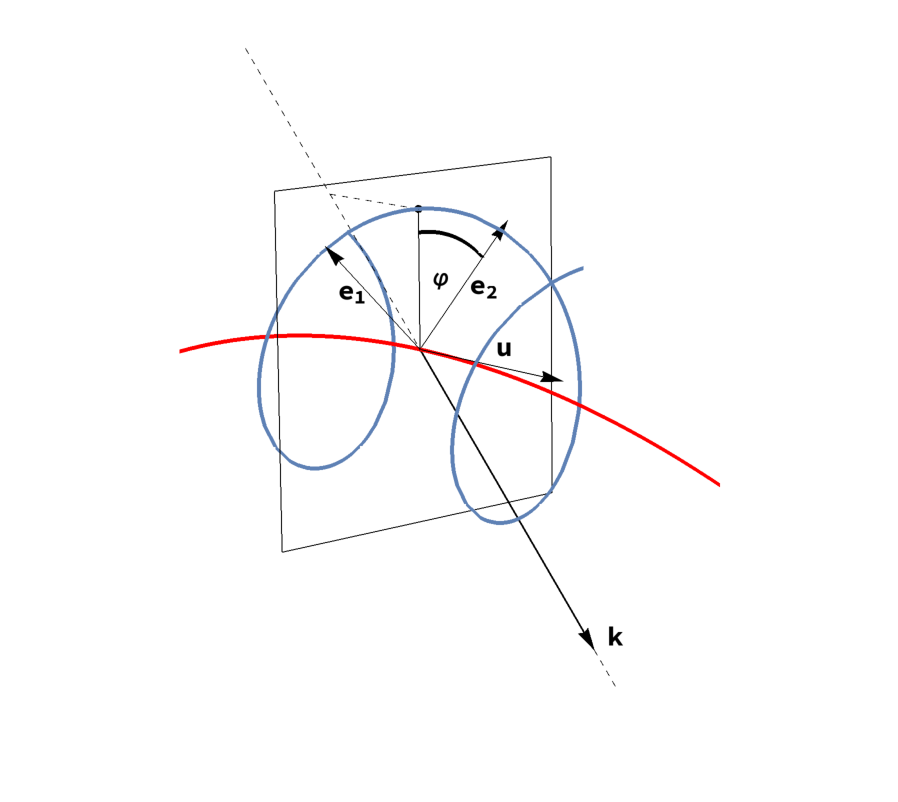
\includegraphics[scale=0.5]{clock.eps}
\caption{Schematyczny rysunek obrazujący działania zegara.}
\label{clock_schemat}
\end{wrapfigure}
Zakładamy, że podczas ruchu mamy spełniony więz~\eqref{wiez}.
Założymy dodatkowo, że wektor zerowy $\dot{x}$ można przedstawić
jako kombinację liniową $e$ oraz $k$ taką, że $e\cdot \dot{x} = 1$.
Rozkładając $\dot{x}$ w bazie $E$ dostajemy
\begin{align*}
\dot{x} = e - C (k\cdot e_1) e_1 - C (k\cdot e_2)e_2.
\end{align*}
Korzystając z faktu, że $\dot{x}$ jest zerowy możemy wyznaczyć
współczynniki kombinacji liniowej.
\begin{align*}
0 = \dot{x} \cdot \dot{x} = 1 - C^2 (k\cdot e_1)^2 - C^2 (k\cdot e_2)^2
= 1 - C^2 (k\cdot e)^2, \\
C= \pm 1/(k\cdot e).
\end{align*}
Wybieramy znak ujemny, gdyż w przeciwnym przypadku
$\dot{x}\cdot k = 0$, co jest sprzeczne z~więzem~\eqref{wiezD}.
 Zatem
\begin{align}
\dot{x} = 2 e - k / (k\cdot e) = 
e + \cos \varphi e_1 + \sin\varphi e_2
,\quad \dot{x}\cdot k = 2 k \cdot e .
\end{align}
Następnie obliczamy pochodną absolutną wektora $k$
\begin{align*}
\dot{k} =\underbrace{ \frac{\d (k\cdot e)}{\d s} e - 
\frac{\d (k\cdot e_1)}{\d s}e_1 -
\frac{\d (k\cdot e_2)}{\d s}e_2}_{K_p}
+\underbrace{(k\cdot e)\dot{e} - (k\cdot e_1)\dot{e_1} 
-(k\cdot e_2)\dot{e_2} }_{K} ,
\end{align*}
\begin{align*}
\dot{k}\cdot\dot{k} = K_p\cdot K_p + K\cdot K + 2K_p\cdot K .
\end{align*}

Obliczamy oddzielnie każdy ze składników powyższej sumy.
Zaczniemy od przedstawienia pochodnych wersorów bazy w bardziej
użytecznej postaci 
\begin{align*}
\dot{e}= \frac{\D e}{\d s} = A,
\end{align*}
\begin{align*}
\dot{e_1}= \frac{\D e_1 }{\d s} = \frac{\D (e_1)_\perp }{\d s} 
\stackrel{\eqref{FW}}{=} 
\left(\frac{\D (e_1)_\perp }{\d s}\cdot e_0\right)e 
= \left(\frac{\D e_1 }{\d s}\cdot e\right)e 
\stackrel{\eqref{FW}}{=} 
 - \left(\frac{\D e }{\d s}\cdot e_1\right)e
= - \left(A\cdot e_1\right)e,
\end{align*}
\begin{align*}
\dot{e_2}= \frac{\D e_2 }{\d s} = \frac{\D (e_2)_\perp }{\d s} 
\stackrel{\eqref{FW}}{=} 
\left(\frac{\D (e_2)_\perp }{\d s}\cdot e\right)e
= \left(\frac{\D e_2 }{\d s}\cdot e\right)e 
\stackrel{\eqref{FW}}{=} 
 - \left(\frac{\D e }{\d s}\cdot e_2\right)e
= - \left(A\cdot e_2\right)e.
\end{align*}

Zgodnie z powyższym zachodzą równości
\begin{align*}
K= (k\cdot e) (A + \left(A\cdot e_1\right)\cos\varphi\ e+ 
\left(A\cdot e_2\right)\sin\varphi\ e ),
\end{align*}
\begin{align*}
K_p= (k\cdot e) \dot{\varphi} ( \sin\varphi\ e_1 - \cos\varphi\ e_2  ) + 
\frac{\d(k\cdot e)}{\d s} (e-\cos\varphi\ e_1 - \sin\varphi\ e_2) ,
\end{align*}

\begin{align*}
K_p\cdot K_p &= \left(  \frac{\d (k\cdot e)}{\d s} \right)^2 
		- \left( \frac{\d (k\cdot e_1)}{\d s} \right)^2 
		- \left( \frac{\d (k\cdot e_2)}{\d s} \right)^2 
		= \left(  \frac{\d (k\cdot e)}{\d s} \right)^2 
		- \left( \frac{\d (k\cdot e)\cos\varphi}{\d s} \right)^2 
		- \left( \frac{\d (k\cdot e)\sin\varphi}{\d s} \right)^2 =
	\\ &= \left(  \frac{\d (k\cdot e)}{\d s} \right)^2 
		- \left( \frac{\d (k\cdot e)}{\d s} 
            \right)^2 (\cos^2\varphi + \sin^2\varphi)
		- (k\cdot e)^2  (\dot{\varphi} )^2 (\sin^2\varphi + \cos^2\varphi) =
	\\ &= - (k\cdot e)^2  (\dot{\varphi} )^2 ,
	\\
	\\
2K_p\cdot K &= 2(k\cdot e_0 ) \dot{\varphi} \left( (A\cdot e_1) 
                \sin\varphi -(A\cdot e_2) \cos\varphi \right) 
        -\frac{\d(k\cdot e_0)}{\d s} \left((A\cdot e_1)\cos\varphi + 
                (A\cdot e_2) \sin\varphi \right)+
    \\ &+\frac{\d(k\cdot e_0)}{\d s} (A\cdot e_1)\cos\varphi 
        +\frac{\d(k\cdot e_0)}{\d s} (A\cdot e_2)\sin\varphi =
    \\ &=2(k\cdot e_0 ) \dot{\varphi} \left( (A\cdot e_1) \sin\varphi -
                (A\cdot e_2) \cos\varphi \right) , 
	\\
	\\
K\cdot K &= (k\cdot e)^2 ( (A\cdot A ) +( \left(A\cdot e_1\right)\cos\varphi+
                    \left(A\cdot e_2\right)\sin\varphi )^2) =
    \\   &=- (k\cdot e)^2( (A\cdot e_1 )^2 + (A\cdot e_2)^2 -
                    (A\cdot e_1)^2\cos^2\varphi - (A\cdot e_2)^2\sin^2\varphi
            - 2 (A\cdot e_1) (A\cdot e_2) \sin\varphi\cos\varphi ) =
    \\   &=- (k\cdot e)^2\left( (A\cdot e_1) \sin\varphi -
                    (A\cdot e_2) \cos\varphi \right)^2 .
\end{align*}
Sumę powyższych składników możemy zwinąć do kwadratu 
\begin{align*}
1 = -\frac{\ell^2\dot{k}\cdot \dot{k}}{(k\cdot \dot{x})^2}  =
\frac{\ell^2}{4} 
( \dot{\varphi} -(A\cdot e_1) \sin\varphi +(A\cdot e_2) \cos\varphi )^2 
\end{align*}
i wyznaczamy
\begin{align*}
\dot{\varphi} = \pm \frac{2}{\ell} +
(A\cdot e_1) \sin\varphi - (A\cdot e_2) \cos\varphi .
\end{align*}
Podstawiając zmienną $\chi$ możemy zapisać owo równanie w 
zgrabnej postaci
%\begin{align*}
%\dot{\varphi}   =\pm \frac{2}{\ell} + \alpha \cos\chi \sin\varphi -
%\alpha \sin\chi \cos\varphi  ,
%\end{align*}
\begin{align}\label{phi_equation}
\boxed{
\dot{\varphi}   = \pm \frac{2}{\ell} +\alpha \sin ( \varphi -\chi ) .
}
\end{align}
W przypadku zerowego przyspieszenia właściwego 
wprowadzony model zegara mierzy czas własny $s$.
\begin{align}
\dot{\varphi} = \frac{2}{\ell},\quad
\varphi =\pm \frac{2}{\ell} s + \varphi_0.
\end{align}
